\documentclass[]{article}
\usepackage{lmodern}
\usepackage{amssymb,amsmath}
\usepackage{ifxetex,ifluatex}
\usepackage{fixltx2e} % provides \textsubscript
\ifnum 0\ifxetex 1\fi\ifluatex 1\fi=0 % if pdftex
  \usepackage[T1]{fontenc}
  \usepackage[utf8]{inputenc}
\else % if luatex or xelatex
  \ifxetex
    \usepackage{mathspec}
  \else
    \usepackage{fontspec}
  \fi
  \defaultfontfeatures{Ligatures=TeX,Scale=MatchLowercase}
\fi
% use upquote if available, for straight quotes in verbatim environments
\IfFileExists{upquote.sty}{\usepackage{upquote}}{}
% use microtype if available
\IfFileExists{microtype.sty}{%
\usepackage{microtype}
\UseMicrotypeSet[protrusion]{basicmath} % disable protrusion for tt fonts
}{}
\usepackage[margin=1in]{geometry}
\usepackage{hyperref}
\hypersetup{unicode=true,
            pdftitle={Identifying Hand Gestures through Myographic Signals via ANN},
            pdfauthor={Sam Voisin, Eduardo Coronado, Sebastian Knigge, Yuan Zheng},
            pdfborder={0 0 0},
            breaklinks=true}
\urlstyle{same}  % don't use monospace font for urls
\usepackage{graphicx,grffile}
\makeatletter
\def\maxwidth{\ifdim\Gin@nat@width>\linewidth\linewidth\else\Gin@nat@width\fi}
\def\maxheight{\ifdim\Gin@nat@height>\textheight\textheight\else\Gin@nat@height\fi}
\makeatother
% Scale images if necessary, so that they will not overflow the page
% margins by default, and it is still possible to overwrite the defaults
% using explicit options in \includegraphics[width, height, ...]{}
\setkeys{Gin}{width=\maxwidth,height=\maxheight,keepaspectratio}
\IfFileExists{parskip.sty}{%
\usepackage{parskip}
}{% else
\setlength{\parindent}{0pt}
\setlength{\parskip}{6pt plus 2pt minus 1pt}
}
\setlength{\emergencystretch}{3em}  % prevent overfull lines
\providecommand{\tightlist}{%
  \setlength{\itemsep}{0pt}\setlength{\parskip}{0pt}}
\setcounter{secnumdepth}{0}
% Redefines (sub)paragraphs to behave more like sections
\ifx\paragraph\undefined\else
\let\oldparagraph\paragraph
\renewcommand{\paragraph}[1]{\oldparagraph{#1}\mbox{}}
\fi
\ifx\subparagraph\undefined\else
\let\oldsubparagraph\subparagraph
\renewcommand{\subparagraph}[1]{\oldsubparagraph{#1}\mbox{}}
\fi

%%% Use protect on footnotes to avoid problems with footnotes in titles
\let\rmarkdownfootnote\footnote%
\def\footnote{\protect\rmarkdownfootnote}

%%% Change title format to be more compact
\usepackage{titling}

% Create subtitle command for use in maketitle
\newcommand{\subtitle}[1]{
  \posttitle{
    \begin{center}\large#1\end{center}
    }
}

\setlength{\droptitle}{-2em}

  \title{Identifying Hand Gestures through Myographic Signals via ANN}
    \pretitle{\vspace{\droptitle}\centering\huge}
  \posttitle{\par}
    \author{Sam Voisin, Eduardo Coronado, Sebastian Knigge, Yuan Zheng}
    \preauthor{\centering\large\emph}
  \postauthor{\par}
      \predate{\centering\large\emph}
  \postdate{\par}
    \date{April 25, 2019}


\begin{document}
\maketitle

\subsection{Abstract}\label{abstract}

\subsection{Introduction}\label{introduction}

Recent advances in surface electromyographic signal (sEMG)
recordingsystems and analytics methods have encouraged the use of sEMGs
in human-machine interfaces to control exoskeletons and protheses;
however, challenges remain. Accurate classification of user movements is
highly variable given the inherent noise of sEMG recording systems and
per-user variability. In turn, this leads to problems downstream when
attempting to convert these classifications into spatial directions
(e.g.~up, down, right, and left). Here, we aim to address the former
challenge specifically. Our goal is to design and implement a
light-weight unsupervised learning model via a multi-layered neural
network to accurately identify six distinct hand gestures from sEMG
data.

\subsection{Methods}\label{methods}

Our analysis workflow was comprised of 4 main phases: preprocessing,
dimension reduction via PCA, modeling, and performance comparison as
shown in Figure 1.

\begin{figure}
\centering
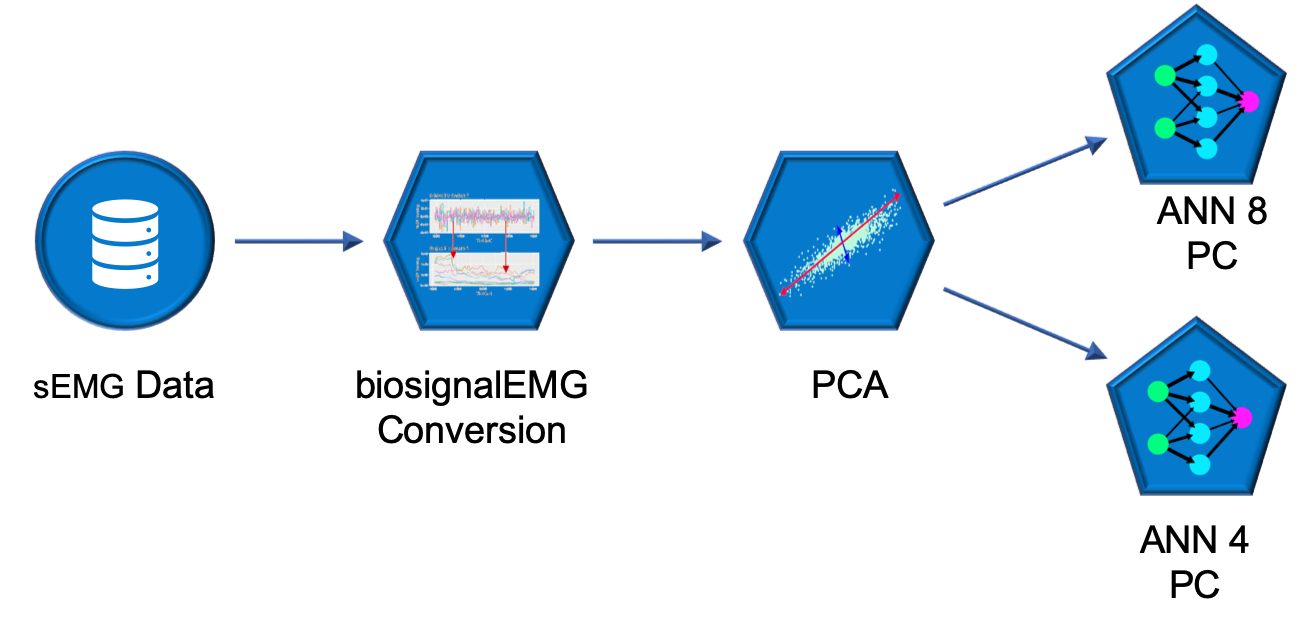
\includegraphics{/Graphics/Flow.png}
\caption{Schematic of overall workflow stages: preprocessing, PCA,
modeling and performance comparison}
\end{figure}

\subsection{Results}\label{results}

\subsection{References}\label{references}


\end{document}
